\section{Question 1}

\begin{question}
    Compute the following two problems with the 2nd order MUSCL scheme.
\end{question}

\subsection{Part a}

\begin{question}
    Problem 3 in H.W. 2.
    
    $$\left\{\begin{array}{l}u_t+u_x=0, \quad t>0, \quad x \in(0,1) \\ u(x, 0)=-\sin (3 \pi x), \text{ if } x \in\left[0, \frac{1}{3}\right) ; \; 1 \text { if } x \in\left[\frac{1}{3}, \frac{2}{3}\right) ; \; 0 \text{ if } x \in\left[\frac{2}{3}, 1\right] \\ u(0, t)=u(1, t), \quad t>0 .\end{array}\right.$$
\end{question}

\begin{answer}
    I used the second order MUSCL scheme in $\MATLAB$ to solve this question. I used the time step of $0.00001$ and location difference of $0.001$. Then, I got the result as in the Figure \ref{fig:fig2}.
    \begin{figure}[H]
        \centering
        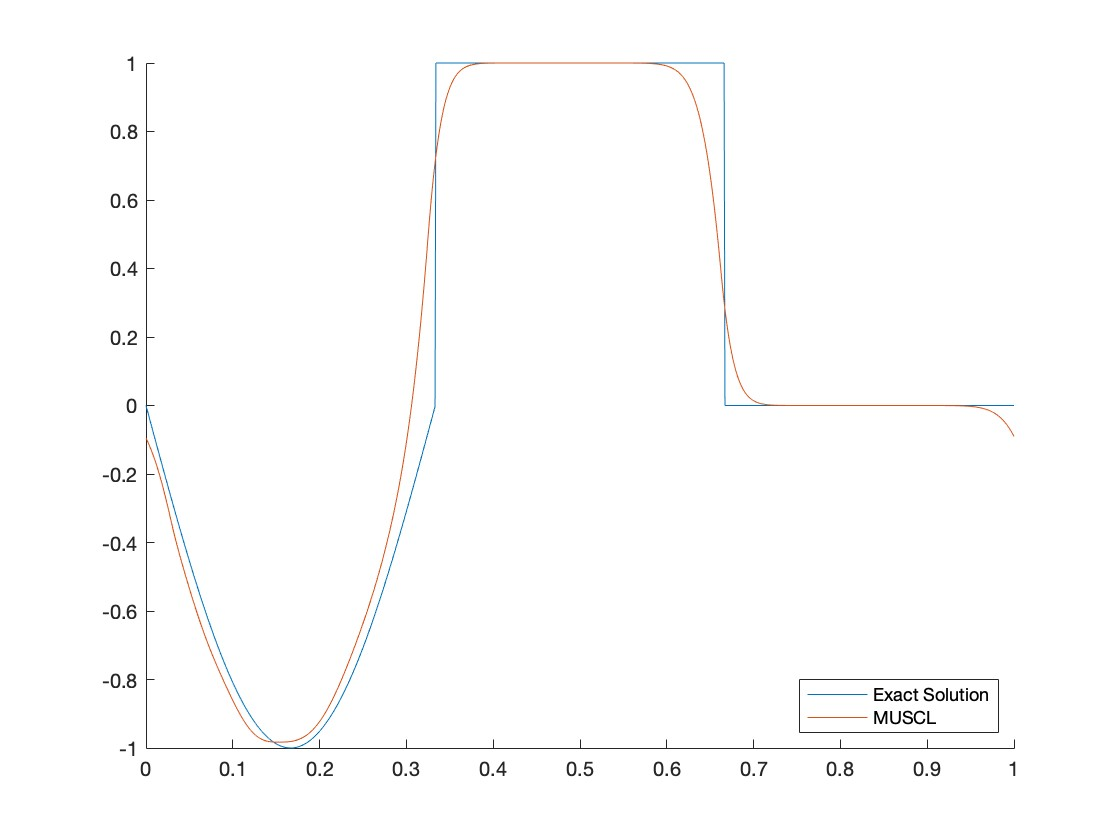
\includegraphics[width=0.99\textwidth]{Result2.jpg}
        \caption{\label{fig:fig2}Exact Solution v.s. Numerical Solution from the MUSCL Scheme at time 10}
    \end{figure}
\end{answer}

\subsection{Part b}

\begin{question}
    $$
    \left\{\begin{array}{l}
    u_t+\left(\frac{1}{2} u^2\right)_x=0, \quad t>0, x \in \mathbb{R} \\
    u(x, 0)=1+\sin (2 \pi x), \quad x \in \mathbb{R} .
    \end{array}\right.
    $$
    The final time is $T=1$.
\end{question}

\begin{answer}
    I used the second order MUSCL scheme in $\MATLAB$ to solve this question. I used the time step of $0.0001$ and location difference of $0.01$. Then, I got the result as in the Figure \ref{fig:fig3}.
    \begin{figure}[H]
        \centering
        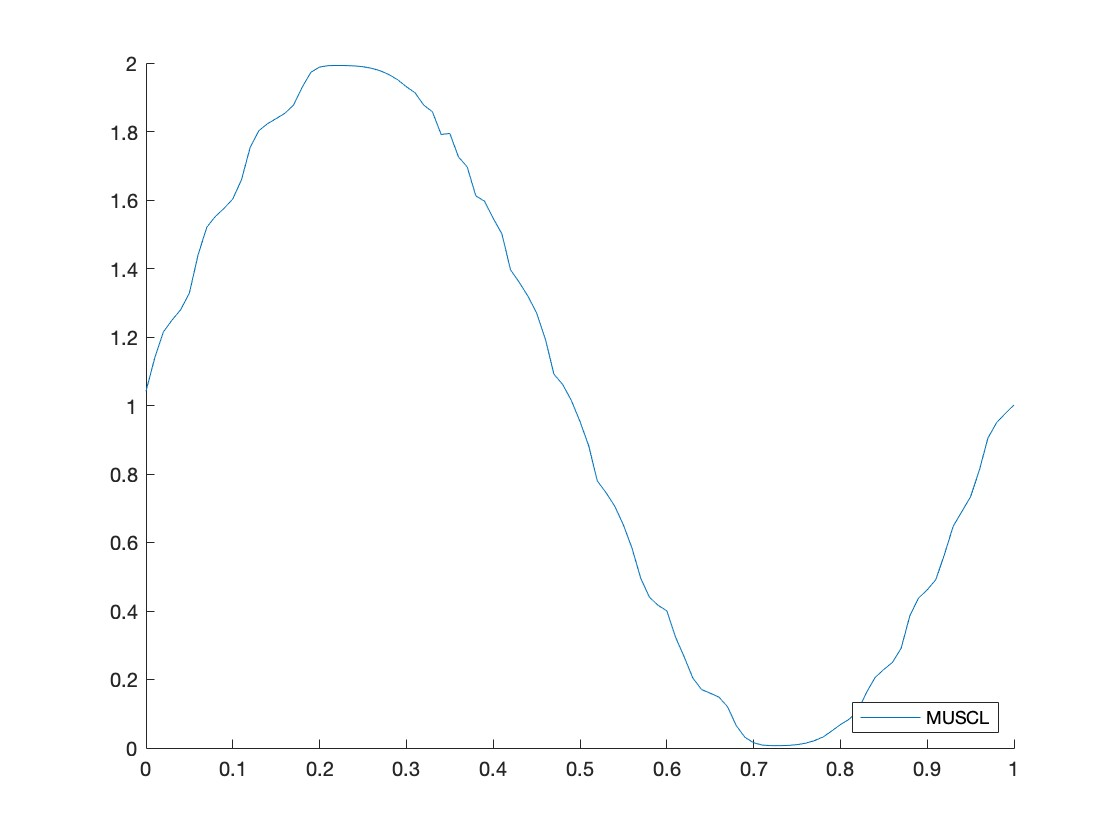
\includegraphics[width=0.99\textwidth]{Result3.jpg}
        \caption{\label{fig:fig3}Solution from the MUSCL Scheme at time 1}
    \end{figure}
\end{answer}